Fitting the anomalous couplings one at a time while fixing the other couplings
to the Standard Model values, we get the following results:

%% Minuit2Minimizer: Minimize with max iterations 3500 edmval 1 strategy 1
%% Minuit2Minimizer : Valid minimum - status = 0
%% FVAL  = -1572.37279032374568
%% Edm   = 8.4141930757717904e-06
%% Nfcn  = 116
%% n_dy	  = 15.0343	 +/-  12.1833	(limited)
%% n_top	  = 97.2587	 +/-  39.9652	(limited)
%% n_wjets	  = 94.1379	 +/-  36.975	(limited)
%% n_ww	  = 878.464	 +/-  69.2675	(limited)
%% n_wz	  = 18.5939	 +/-  3.71088	(limited)
%% n_zz	  = 10.5644	 +/-  1.95431	(limited)
%% x_par	  = 0.0052845	 +/-  0.0458341	(limited)
%% Info in <Minuit2>: MnMinos Parameter is at Lower limit. : par = 0
%% Minos:  Parameter  is at Lower limit.
%% Minos: Lower error for parameter 0  :  -12.1093
%% Minos: Upper error for parameter 0  :  13.1484
%% Minos: Lower error for parameter 1  :  -40.2918
%% Minos: Upper error for parameter 1  :  40.4678
%% Minos: Lower error for parameter 2  :  -37.3677
%% Minos: Upper error for parameter 2  :  37.6453
%% Minos: Lower error for parameter 3  :  -68.9822
%% Minos: Upper error for parameter 3  :  69.6025
%% Minos: Lower error for parameter 4  :  -3.72124
%% Minos: Upper error for parameter 4  :  3.72263
%% Minos: Lower error for parameter 5  :  -1.95916
%% Minos: Upper error for parameter 5  :  1.95939
%% Minos: Lower error for parameter 6  :  -0.0418783
%% Minos: Upper error for parameter 6  :  0.0356141
%% [#1] INFO:Minization --  Including the following contraint terms in minimization: (n_ww_con,n_top_con,n_wjets_con,n_wz_con,n_zz_con,n_dy_con)
%% [#1] INFO:Fitting -- RooAddition::defaultErrorLevel(nll_cpdf_data_with_constr) Summation contains a RooNLLVar, using its error level
%% Minuit2Minimizer: Minimize with max iterations 3500 edmval 1 strategy 1
%% Minuit2Minimizer : Valid minimum - status = 0
%% FVAL  = -1572.36968234415076
%% Edm   = 2.0952445060625156e-05
%% Nfcn  = 90
%% n_dy	  = 15.0668	 +/-  12.181	(limited)
%% n_top	  = 97.4828	 +/-  39.897	(limited)
%% n_wjets	  = 94.2751	 +/-  36.9723	(limited)
%% n_ww	  = 878.745	 +/-  69.3521	(limited)
%% n_wz	  = 18.5961	 +/-  3.71081	(limited)
%% n_zz	  = 10.5652	 +/-  1.95429	(limited)
%% y_par	  = 0.00759402	 +/-  0.0725263	(limited)
%% Info in <Minuit2>: MnMinos Parameter is at Lower limit. : par = 0
%% Minos:  Parameter  is at Lower limit.
%% Minos: Lower error for parameter 0  :  -12.1418
%% Minos: Upper error for parameter 0  :  13.123
%% Minos: Lower error for parameter 1  :  -40.175
%% Minos: Upper error for parameter 1  :  40.4237
%% Minos: Lower error for parameter 2  :  -37.4662
%% Minos: Upper error for parameter 2  :  37.5493
%% Minos: Lower error for parameter 3  :  -68.8703
%% Minos: Upper error for parameter 3  :  69.8972
%% Minos: Lower error for parameter 4  :  -3.72284
%% Minos: Upper error for parameter 4  :  3.72104
%% Minos: Lower error for parameter 5  :  -1.9595
%% Minos: Upper error for parameter 5  :  1.95905
%% Minos: Lower error for parameter 6  :  -0.0652585
%% Minos: Upper error for parameter 6  :  0.059694
%% [#1] INFO:Minization --  Including the following contraint terms in minimization: (n_ww_con,n_top_con,n_wjets_con,n_wz_con,n_zz_con,n_dy_con)
%% [#1] INFO:Fitting -- RooAddition::defaultErrorLevel(nll_cpdf_data_with_constr) Summation contains a RooNLLVar, using its error level
%% Minuit2Minimizer: Minimize with max iterations 3500 edmval 1 strategy 1
%% Minuit2Minimizer : Valid minimum - status = 0
%% FVAL  = -1579.3847460662123
%% Edm   = 4.26748276886769417e-06
%% Nfcn  = 108
%% n_dy	  = 13.5107	 +/-  12.1214	(limited)
%% n_top	  = 105.896	 +/-  39.3617	(limited)
%% n_wjets	  = 86.9187	 +/-  37.2819	(limited)
%% n_ww	  = 879.761	 +/-  69.0987	(limited)
%% n_wz	  = 18.5643	 +/-  3.71085	(limited)
%% n_zz	  = 10.5782	 +/-  1.95426	(limited)
%% y_par	  = 0.0187651	 +/-  0.171486	(limited)
%% Info in <Minuit2>: MnMinos Parameter is at Lower limit. : par = 0
%% Minos:  Parameter  is at Lower limit.
%% Minos: Lower error for parameter 0  :  -10.5857
%% Minos: Upper error for parameter 0  :  13.1729
%% Minos: Lower error for parameter 1  :  -39.583
%% Minos: Upper error for parameter 1  :  39.8618
%% Minos: Lower error for parameter 2  :  -37.8626
%% Minos: Upper error for parameter 2  :  37.895
%% Minos: Lower error for parameter 3  :  -68.7551
%% Minos: Upper error for parameter 3  :  69.5066
%% Minos: Lower error for parameter 4  :  -3.72228
%% Minos: Upper error for parameter 4  :  3.72167
%% Minos: Lower error for parameter 5  :  -1.9594
%% Minos: Upper error for parameter 5  :  1.95907
%% Minos: Lower error for parameter 6  :  -0.183209
%% Minos: Upper error for parameter 6  :  0.129282

%% \begin{align}
%%   \lambda_{Z} &= 0.00\pm0.19, ~95\%~\mathrm{C.L.} \\ 
%%   \Delta g^Z_1 &= 0.01\pm0.30, ~95\%~\mathrm{C.L.}\\
%%   \Delta\kappa_\gamma &= 0.02\pm0.63, ~95\%~\mathrm{C.L.}\\
%% \end{align}

%% \fixme{What do we do with coverage? Ignore for now}

%% Sampling \wwll\ Monte Carlo events we find that within the reported 95\%
%% confidence limits $\lambda_{Z}$ contained $97\pm1$\% and
%% $\Delta\kappa_{Z}$ contained $94\pm1$\% of the test samples.

Systematic uncertainties were included in the fit as Gaussian
constraints.

Final exclusion limits for anomalous couplings are:
\begin{align}
  \lambda_{Z}: [-0.046,0.051]~95\%~\mathrm{C.L.}\\ 
  \Delta g^{Z}_1: [-0.077,0.092]~95\%~\mathrm{C.L.}\\
  \Delta\kappa_\gamma: [-0.23,0.21]~95\%~\mathrm{C.L.}\\
\end{align}
The results include the scale correction of 20-30\% observed in the validation studies.

Figure~\ref{fig:contour} shows 2D confidence limit contour plots for
anomalous couplings.

\begin{figure}[tp]
  \centering
    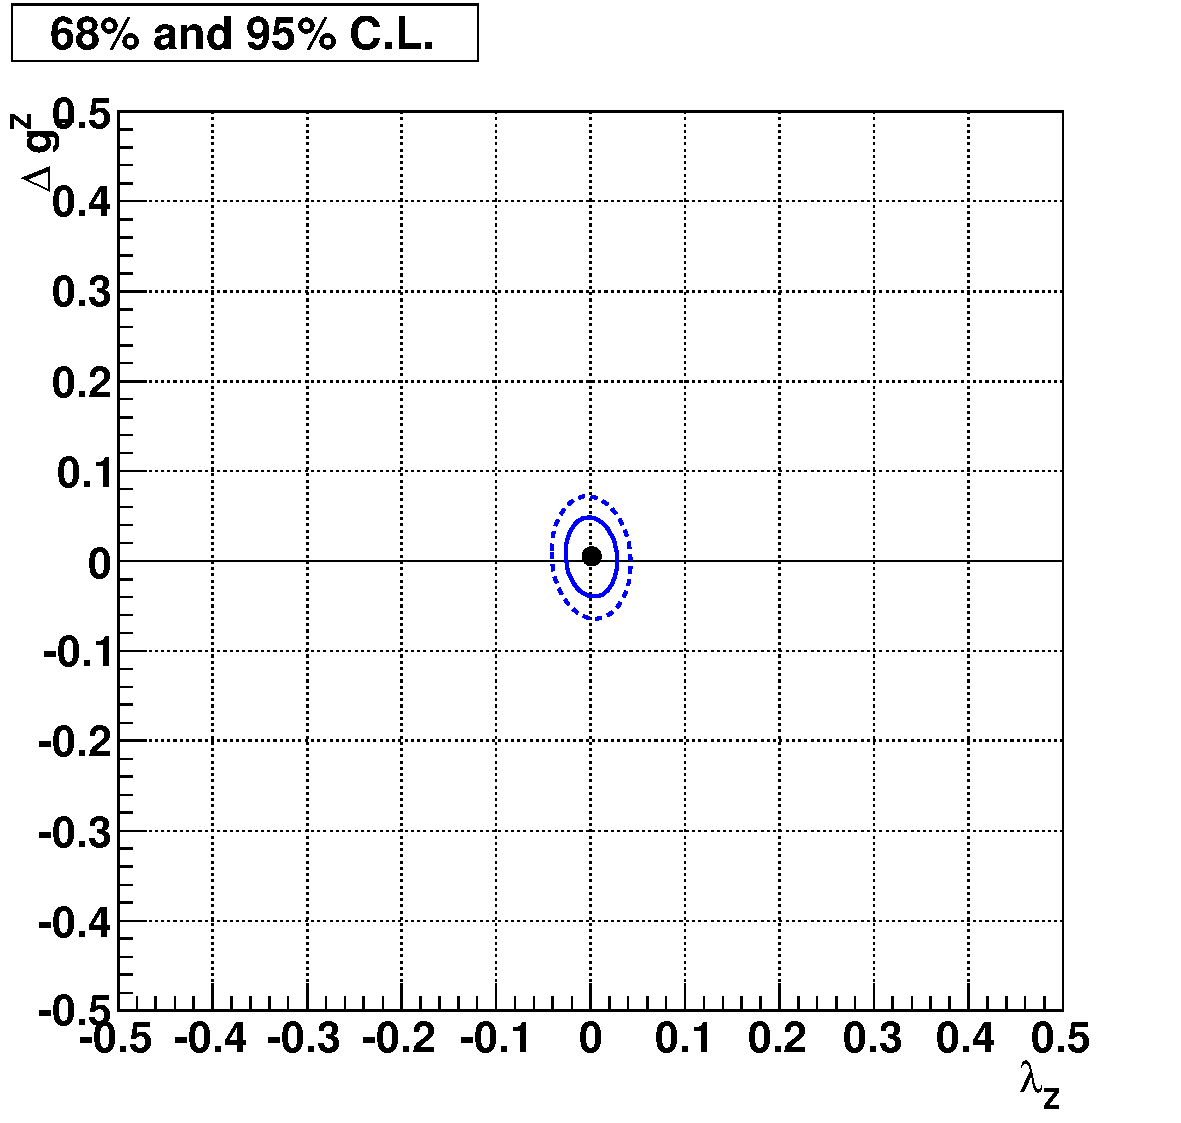
\includegraphics[width=0.7\textwidth]{figures/lz_dgz_contourplot}
    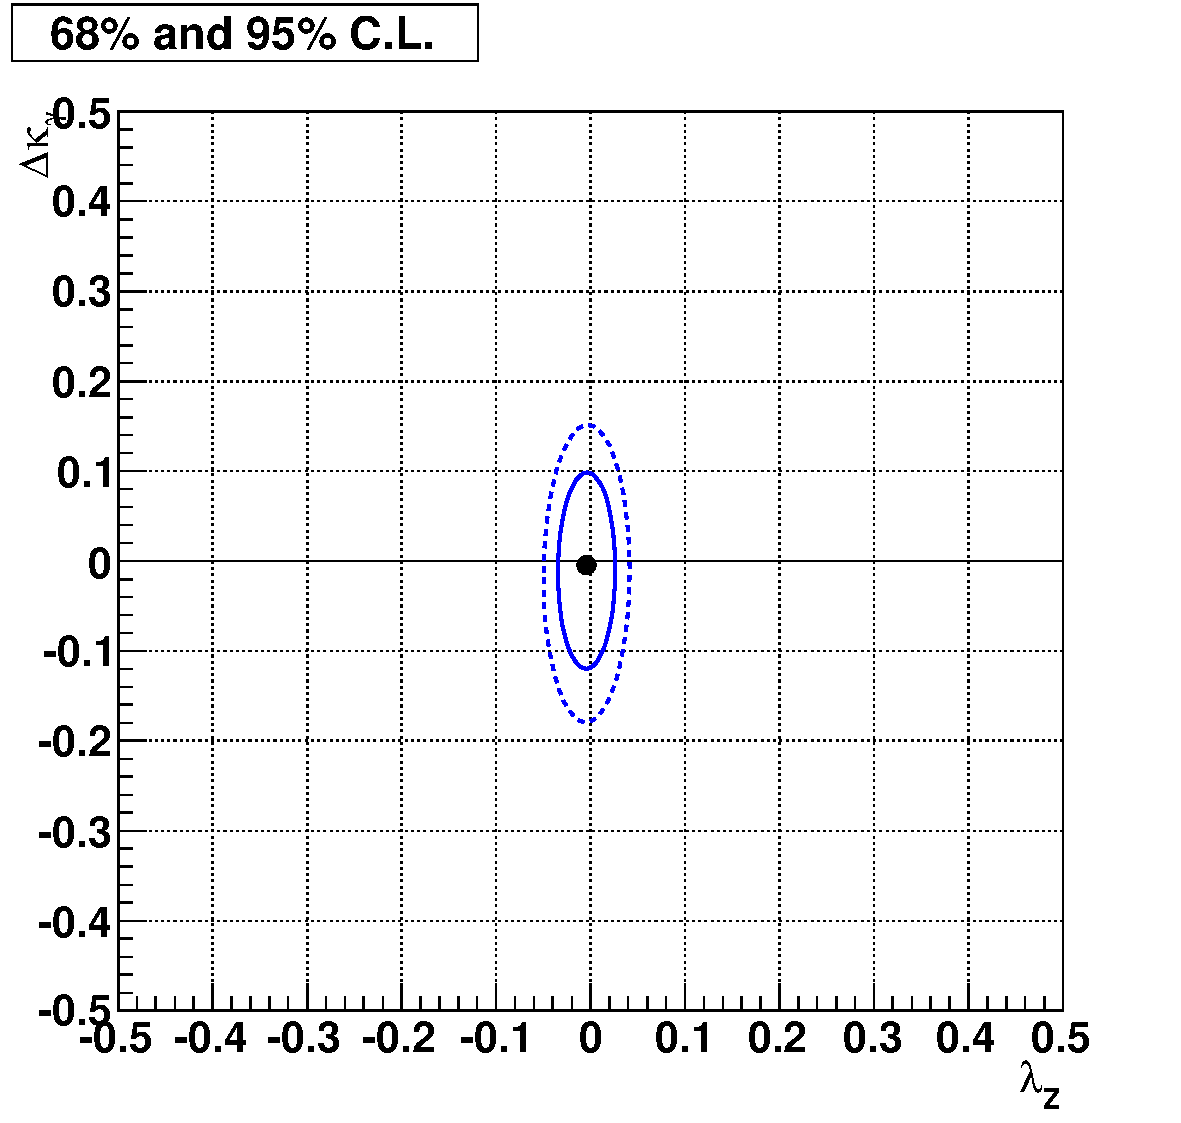
\includegraphics[width=0.7\textwidth]{figures/lz_dkg_contourplot}
  

  \caption[Contour plots for data] {aTGC 68\% and 95\% C.L. contour
    plots for a model without form factors for \intlumi of data.}
  \label{fig:contour}
\end{figure}

